\chapter{基于概率阅读的事件传播模型研究}
\label{chap5:main}
信息传播的\textbf{信息传播模型}分析是社交网络分析中的一个重要研究点,网络热点事件通过社交网络平台迅速传播、发酵,从而在短时间内形成信息爆发、造成极大的影响。社交网络加速了新闻、通知等信息的传播,使得人们接受信息的速率加快,传播信息的成本降低,在一定程度上方便了人们的生活。但是,在社交网络中,人人都可以是信息的生产者、传播者和接收者,每一个社交网络用户都能通过平台发布传播信息。在社交网络中制造舆论热点,进行信息传播的代价相对于传统媒体较低,因此很容易被不法分子利用,对社会安全以及人身财产等造成损失。已有的信息传播模型研究主要包括独立级联模型和线性阈值模型等,这些模型对信息的传播进行了量化,对信息的传播范围进行了传播范围的评估。但是,仍然有一些需求在实际应用中得不到满足。

在信息传播过程中,一个被激活的节点(信息接收者)将尝试继续传播该信息,去激活下一个节点,从而产生级联效应。在实际应用中,一个事件往往由多条主要的信息组成,因此一个事件的传播将由多个传播网络组合而成。所以事件的传播模型首先需要考虑的是多个传播网络的融合问题。其次,社交网络中存在很多的垃圾用户,这些用户活跃度低,或者是由水军控制,会影响到影响力量化的计算,因此需要建立垃圾用户过滤的机制,除去这些干扰噪声。最后,信息的叶子节点,即事件传播的最终的接收者(不再进行下一轮传播)是否阅读到了该信息是概率性的,因此根据用户的社交行为来为用户阅读信息进行建模能够提高影响力量化的准确度。出于精确量化事件传播的影响力的需求,本章提出了一个基于概率阅读的事件传播模型,将多信息传播网络融合、垃圾用户过滤和概率阅读模型综合考虑,为事件在社交网络中的传播进行建模,精确量化事件的传播影响力。

本章的主要工作可以总结如下。首先,基于事件中单条信息的传播网络,我们对多个传播网络进行融合,去除掉重复的节点。其次,利用用户在社交网络中的社交属性,基于逻辑回归模型进行建模,使用梯度下降法进行参数训练,最终得到模型用于垃圾用户过滤。然后,利用用户在社交网络中的时间线上的社交属性,对用户阅读到信息的概率进行建模,对概率阅读模型进行参数训练,得到的模型最终用来预测用户阅读到信息的概率。最后,本章对提出的模型进行了验证,实验使用新浪微博的真实数据集,实验结果证明了模型的有效性。

本章的内容组织如下:第\ref{sec5:motivation}节介绍本章的研究动机,讨论了传统的传播模型的不足之处以及研究基于概率阅读的事件传播模型的意义。第\ref{sec5:definition}节介绍了相关的定义,对本章中所研究的问题进行了定义。第\ref{sec5:method}节介绍了方法描述,详细地阐述了本章提出的模型以及建立过程。第\ref{sec5:experiment}节进行了实验分析,通过实验结果验证了模型的正确性,并对实验结果进行了分析。最后,第\ref{sec5:conclusion}节对本章进行了总结。
\section{研究动机}
\label{sec5:motivation}
在Web 2.0时代,社交网络媒介逐渐开始取代如同报刊、杂志、新闻等传统媒介,占据了信息传播的主导位置。随着各大社交网站的发展,如国外的脸书(Facebook)、推特(Twitter)等,国内的新浪微博、腾讯微博等。与此同时,传统媒介也开始结合社交网络媒介,纷纷开设自己的公共主页,通过互联网及时发布信息,将信息在第一时间推送给用户。在不如大数据时代后,各大社交网络门户的用户呈现几何式爆炸增长的趋势,一条信息通过网络平台在短时间内能够传播影响到的数以百万计的用户。相比于传统媒介,社交网络媒介在信息传播过程中的传播效率与传播范围都大大增强,然而一些虚假信息通过社交网络媒介的传播也能在短时间内迅速扩散,从而可能造成社会的恐慌、用户财产的损失等问题。因此,在大数据时代,社交网络媒介中的信息传播问题成为了信息安全领域的一个研究热点。

信息传播模型定义了社交网络中影响力传播的方式和机制,是研究社交网络中事件传播影响的基础。已有的研究对传播模型做出了深入的研究,其中广泛应用的模型主要有\textbf{独立级联模型}(\textit{Independent Cascade Model})\upcite{goldenberg2001talk,Goldenberg2001Using}和\textbf{线性阈值模型}(\textit{Linear Threshold Model})\upcite{Granovetter1986Threshold,granovetter1983threshold},这两种模型分别从不同的角度描述了信息传播的过程。

独立级联模型是一种概率传播模型,源于市场营销模型研究。独立级联模型基于概率,每一个传播节点在自身转变为活跃状态后,都可以以一定的概率取激活其后继节点,并且多个活跃节点试图影响同一个邻居节点的事件是独立的,所以称之为独立级联模型。独立级联模型是一种比较经典的模型,适用范围广,能够诠释大多数情况的信息传播过程。

线性阈值模型主要源于节点的特异性研究,模型核心出发点为节点的激活阈值,多个活跃节点试图影响同一后继节点的过程是非独立的,节点激活的成功与否取决于多个节点的加权影响是否超过后继节点的阈值。线性阈值模型体现了信息传播过程中影响的累积效应特性,即节点对后继节点的影响是多个节点的累积。

除了上述的信息传播模型外,目前还有一些其他的信息传播模型研究。最为简单的模型是\textbf{统一模型}(\textit{Uniform Model}),模型假设所有节点的传播影响概率都是一个常数,例如0.01。该模型不考虑节点之间的关系,即边的关系。所有的节点对其邻居节点的影响是相同的,不根据结构的变化而变化。此外,模型还假设一个节点对于其所有的邻居节点的影响也是相同的,即不区分邻居节点之间的差别。很显然,这两个假设在实际应用中都是不能得到满足的。基于统一模型的改进为\textbf{三态模型}(\textit{Trivalency Model}),该模型对统一模型中的第一个假设进行了修正。三态模型不再假设所有的节点的传播影响概率是相同的,节点的传播影响概率是均匀随机地从预先设置的概率集合中选取,例如$\{0.001,0.01,0.1\}$。在统一模型中,每一个节点的传播影响概率是相同的,不可区分的。而在三态模型中,节点的传播影响概率是不同的,是可区分的。三态模型的核心思想是将节点的传播影响概率进行了区分,例如传播影响概率为0.001的节点对应于低影响力的节点,传播影响概率为0.01的节点对应于中影响力的节点,传播影响概率为0.1的节点对应于高影响力的节点。在统一模型和三态模型中,节点的传播影响概率都与网络的结构不相关。在\textbf{加权独立级联模型}(\textit{Weighted Independent Cascade})中,传播影响概率与网络的边相关,即与用户关系相关。传播影响概率定义为$p_{u,v}=1 / d_{in}\left(v\right)$,其中$d_{in}\left(v\right)$为节点$v$的入度。该模型相比于上述的两种模型能够更好地诠释信息在社交网络中的传播过程,对于网络中的节点进行了深层次的区分。入度小的节点受到每个入读邻居节点的影响要大于入度大的节点受到的影响,传播影响概率不是简单地从一个常数集合中选取,而是与网络结构相关。另一方面,节点对于其出度邻居节点的传播影响概率不一定是相同的,这是由于出度邻居节点的入度不同。尽管加权独立级联模型拥有以上良好的特性,然而模型的传播影响概率的计算方法仍然缺乏理论保证,传播影响概率与网络的结构相关,但是没有考虑节点之间的历史传播影响概率。\textbf{选举模型}(\textit{Voter Model})\upcite{evendar2011a}是一种广泛应用在统计物理和粒子系统中的一种模型。在选举模型中,各节点随机选取其某一个前驱节点的状态作为自己的状态。上述的各种模型都对信息传播过程的特点进行了研究和建模,为传播分析提供了理论依据,奠定了研究基础。

在社交网络中,独立级联模型最为适应于社交网络的特性。以微博为例,信息的发布源为某个用户,称之为博主。博主发布的博文将推送至博主所有的粉丝,而粉丝接收到此信息后,将以一定的概率转化为激活状态(即转发此条博文)。如果粉丝转发了博文,则其粉丝又会接收到该信息,进而产生级联效应,促使更多的用户接收到该信息。

社交网络具有自身的特性,特别是进入大数据时代后,平台中的信息量庞大。网络中的节点接收到前驱节点信息的概率与该节点所有的前驱节点的状态有关。以微博为例,用户是否能够接收到其关注用户的信息取决于用户在信息推送时是否处于在线状态,即用户接收信息的概率与信息推送时间和用户在线时间的间隔有关。同时在社交网络中,一些节点的活跃度低,为无效节点,不能将其统计入全局的影响传播中。例如,微博中存在很多的垃圾用户,在计算事件的传播影响力时,需要将其滤出才能还原真实的信息传播过程。传统的信息传播分析主要针对单条博文,而在实际应用中,微博中的一个热点事件往往由多条博文组成。因此,对于事件进行传播分析需要针对多个博文进行分析,对应于信息传播过程中多个信息源的热点。同时,用户阅读到信息的概率与信息的发布时间和接收用户的在线时间的间隔相关,需要建立阅读模型来模拟信息传播过程中特性。本章将针对传统的信息传播模型中存在的不足以及在实际应用中的缺陷,结合多源传播网络融合、垃圾用户过滤和概率阅读模型来进行事件的传播分析。
\section{相关定义}
\label{sec5:definition}
在本小节中,我们对所研究的问题进行详细的描述,并对涉及到的概念进行定义和解释。
\subsection{社交网络的基本定义}
\label{subsec5:socialNetwork}
社交网络是由社会个体成员以及社会个体成员之间的联系组成的一种复杂的关系网络。在相关的社交网络研究中,社交网络通常用图$\mathcal{G}=\left(\mathcal{V},\mathcal{E},\mathcal{W}\right)$来表示。其中节点集合$\mathcal{V}=\{v_1,v_2,\cdots,v_n\}$表示社交网络中的社会个体成员,$n$表示整个网络中个体成员的数目。各个社会个体成员之间的关系由图$\mathcal{G}$的边的集合表示,即$\mathcal{E} \subseteq \mathcal{V} \times \mathcal{V}$,其中$\mathcal{V} \times \mathcal{V}$表示节点的笛卡尔集。社会个体成员之间的关系可以是价值观、合作、关联、亲属、好友等各种类型的关系。社会个体的权重以$\mathcal{W}=\{w_1,w_2,\cdots,w_n\}$来表示,用于表示社会个体成员的重要性,例如影响力、公信力等等特征。

\begin{figure}[!ht]
    \centering
    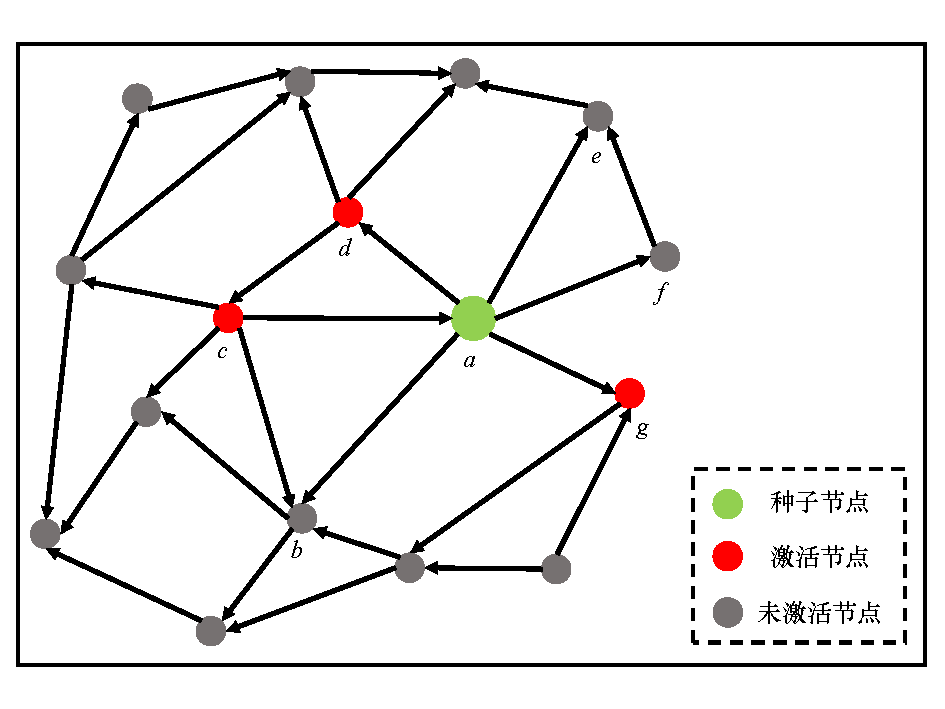
\includegraphics[width=0.8\textwidth]{infoSocial}
    \caption{社交网络中信息传播示意图}
    \label{fig:infoSocial}
\end{figure}

图\ref{fig:infoSocial}给出了社交网络的结构以及信息传播的示意图。信息传播过程可以形式化地描述如下,社交网络中的节点存在两种状态,激活与未激活。在独立级联模型下,给定种子节点后,种子节点首先被激活,然后会以一定概率去激活其他节点,进而形成级联效应。即当节点$u$被激活后,状态由未激活转变成激活,然后节点$u$会以一定的概率去激活处于未激活状态下的邻居节点。如若激活成功,则邻居节点将由未激活状态转变为激活状态,并具备传播能力。如图\ref{fig:infoSocial}中所示,节点$a$为种子节点,在信息传播一开始时被激活,节点$a$在被激活后将以一定的概率去激活其邻居节点$b$、$d$、$e$、$f$、$g$。假设传播情况如图中所示,节点$c$、$d$、$g$被激活,节点$e$、$f$未被激活。由为激活状态转变成激活状态这一过程是不可逆的,这种由未激活状态转变成激活状态的过程称之为信息传播过程。

在社交网络中用户之间的关系主要分为两种,有向关系与无向关系。有向关系表示节点与节点之间的关系是有向的,例如新浪微博、推特中的关注关系。无向关系表示节点与节点之间的关系是无向的,例如脸书中的好友关系。二者的不同之处在于有向图中节点与节点的关系是单向的,可以用有向图表示。而无向关系中节点与节点之间的关系是双向的,可以用无向图表示。特别地,无向关系可以用双向的有向关系来表示。例如,如果节点$u$关注节点$v$,但是节点$v$不一定关注节点$u$。如果节点$u$与节点$v$是好友关系,则节点$v$与节点$u$也是好友。在社交网络中,这两种关系都普遍出现,可以用不同的图结构来表示。

\subsection{独立级联模型}
\label{subsec5:icModel}
Gruhl等人首先信息传播模型的传播概率的学习进行了研究,Saito等人\upcite{saito2008prediction}研究了独立级联模型下的信息传播概率。独立级联模型中各个节点之间的影响是相互独立的,每个节点成为激活节点后都有一定的概率来激活其邻居节点。多个节点对同一个节点的激活是相互独立的。

在给定一个初始种子节点集合$S$后,在独立级联模型下信息传播的过程如下所示。在时刻$t=0$,社交网络中节点仅有集合$S$中的节点被激活,其余的节点为非激活状态。如果节点$u$在在时刻$t$被激活,则节点$u$由未激活状态转变成激活状态。在$t+1$时刻,节点$u$将有能力激活其后继节点。假设节点$u$存在一个后继节点$v$,令节点$u$激活节点$v$的概率为$p_{u,v}$。如果节点$u$在$t+1$时刻成功激活节点$v$,则节点$v$由未激活状态变成激活状态,在$t+2$时刻,节点$v$将有能力去激活其后继节点。如果节点$v$未被激活,则会保持未激活状态,但是节点$v$可能在未来的时刻由其他的前继节点激活。信息传播过程将持续到没有节点被激活的时刻为止。

假设$\mathcal{G}=\left(\mathcal{V},\mathcal{E}\right)$为一个社交网络。定义\textbf{信息传播时序}(\textit{information diffusion episode})为一个时间序列$\langle D\left(0\right), D\left(1\right), \cdots, D\left(T\right) \rangle$,且满足条件$D\left(i\right) \cap D\left(j\right) = \emptyset$。其中$T$代表着整个信息传播过程的持续时间,$D\left(t\right)$表示在时间$t$时刻被激活的节点集合。$D\left(0\right)$表示在时间$t=0$时刻被激活的节点,即初始的种子节点集合。约束$D\left(i\right) \cap D\left(j\right) = \emptyset$保证了已经激活的节点不会再变成未激活状态。信息传播过程将持续到$T$时刻结束,其中$D\left(T\right) = \emptyset$,即没有新的节点被激活时,信息传播过程结束。
\section{方法描述}
\label{sec5:method}

\section{实验分析}
\label{sec5:experiment}

\section{本章小结}
\label{sec5:conclusion}